\documentclass[1p]{elsarticle_modified}
%\bibliographystyle{elsarticle-num}

%\usepackage[colorlinks]{hyperref}
%\usepackage{abbrmath_seonhwa} %\Abb, \Ascr, \Acal ,\Abf, \Afrak
\usepackage{amsfonts}
\usepackage{amssymb}
\usepackage{amsmath}
\usepackage{amsthm}
\usepackage{scalefnt}
\usepackage{amsbsy}
\usepackage{kotex}
\usepackage{caption}
\usepackage{subfig}
\usepackage{color}
\usepackage{graphicx}
\usepackage{xcolor} %% white, black, red, green, blue, cyan, magenta, yellow
\usepackage{float}
\usepackage{setspace}
\usepackage{hyperref}

\usepackage{tikz}
\usetikzlibrary{arrows}

\usepackage{multirow}
\usepackage{array} % fixed length table
\usepackage{hhline}

%%%%%%%%%%%%%%%%%%%%%
\makeatletter
\renewcommand*\env@matrix[1][\arraystretch]{%
	\edef\arraystretch{#1}%
	\hskip -\arraycolsep
	\let\@ifnextchar\new@ifnextchar
	\array{*\c@MaxMatrixCols c}}
\makeatother %https://tex.stackexchange.com/questions/14071/how-can-i-increase-the-line-spacing-in-a-matrix
%%%%%%%%%%%%%%%

\usepackage[normalem]{ulem}

\newcommand{\msout}[1]{\ifmmode\text{\sout{\ensuremath{#1}}}\else\sout{#1}\fi}
%SOURCE: \msout is \stkout macro in https://tex.stackexchange.com/questions/20609/strikeout-in-math-mode

\newcommand{\cancel}[1]{
	\ifmmode
	{\color{red}\msout{#1}}
	\else
	{\color{red}\sout{#1}}
	\fi
}

\newcommand{\add}[1]{
	{\color{blue}\uwave{#1}}
}

\newcommand{\replace}[2]{
	\ifmmode
	{\color{red}\msout{#1}}{\color{blue}\uwave{#2}}
	\else
	{\color{red}\sout{#1}}{\color{blue}\uwave{#2}}
	\fi
}

\newcommand{\Sol}{\mathcal{S}} %segment
\newcommand{\D}{D} %diagram
\newcommand{\A}{\mathcal{A}} %arc


%%%%%%%%%%%%%%%%%%%%%%%%%%%%%5 test

\def\sl{\operatorname{\textup{SL}}(2,\Cbb)}
\def\psl{\operatorname{\textup{PSL}}(2,\Cbb)}
\def\quan{\mkern 1mu \triangleright \mkern 1mu}

\theoremstyle{definition}
\newtheorem{thm}{Theorem}[section]
\newtheorem{prop}[thm]{Proposition}
\newtheorem{lem}[thm]{Lemma}
\newtheorem{ques}[thm]{Question}
\newtheorem{cor}[thm]{Corollary}
\newtheorem{defn}[thm]{Definition}
\newtheorem{exam}[thm]{Example}
\newtheorem{rmk}[thm]{Remark}
\newtheorem{alg}[thm]{Algorithm}

\newcommand{\I}{\sqrt{-1}}
\begin{document}

%\begin{frontmatter}
%
%\title{Boundary parabolic representations of knots up to 8 crossings}
%
%%% Group authors per affiliation:
%\author{Yunhi Cho} 
%\address{Department of Mathematics, University of Seoul, Seoul, Korea}
%\ead{yhcho@uos.ac.kr}
%
%
%\author{Seonhwa Kim} %\fnref{s_kim}}
%\address{Center for Geometry and Physics, Institute for Basic Science, Pohang, 37673, Korea}
%\ead{ryeona17@ibs.re.kr}
%
%\author{Hyuk Kim}
%\address{Department of Mathematical Sciences, Seoul National University, Seoul 08826, Korea}
%\ead{hyukkim@snu.ac.kr}
%
%\author{Seokbeom Yoon}
%\address{Department of Mathematical Sciences, Seoul National University, Seoul, 08826,  Korea}
%\ead{sbyoon15@snu.ac.kr}
%
%\begin{abstract}
%We find all boundary parabolic representation of knots up to 8 crossings.
%
%\end{abstract}
%\begin{keyword}
%    \MSC[2010] 57M25 
%\end{keyword}
%
%\end{frontmatter}

%\linenumbers
%\tableofcontents
%
\newcommand\colored[1]{\textcolor{white}{\rule[-0.35ex]{0.8em}{1.4ex}}\kern-0.8em\color{red} #1}%
%\newcommand\colored[1]{\textcolor{white}{ #1}\kern-2.17ex	\textcolor{white}{ #1}\kern-1.81ex	\textcolor{white}{ #1}\kern-2.15ex\color{red}#1	}

{\Large $\underline{12n_{0218}~(K12n_{0218})}$}

\setlength{\tabcolsep}{10pt}
\renewcommand{\arraystretch}{1.6}
\vspace{1cm}\begin{tabular}{m{100pt}>{\centering\arraybackslash}m{274pt}}
\multirow{5}{120pt}{
	\centering
	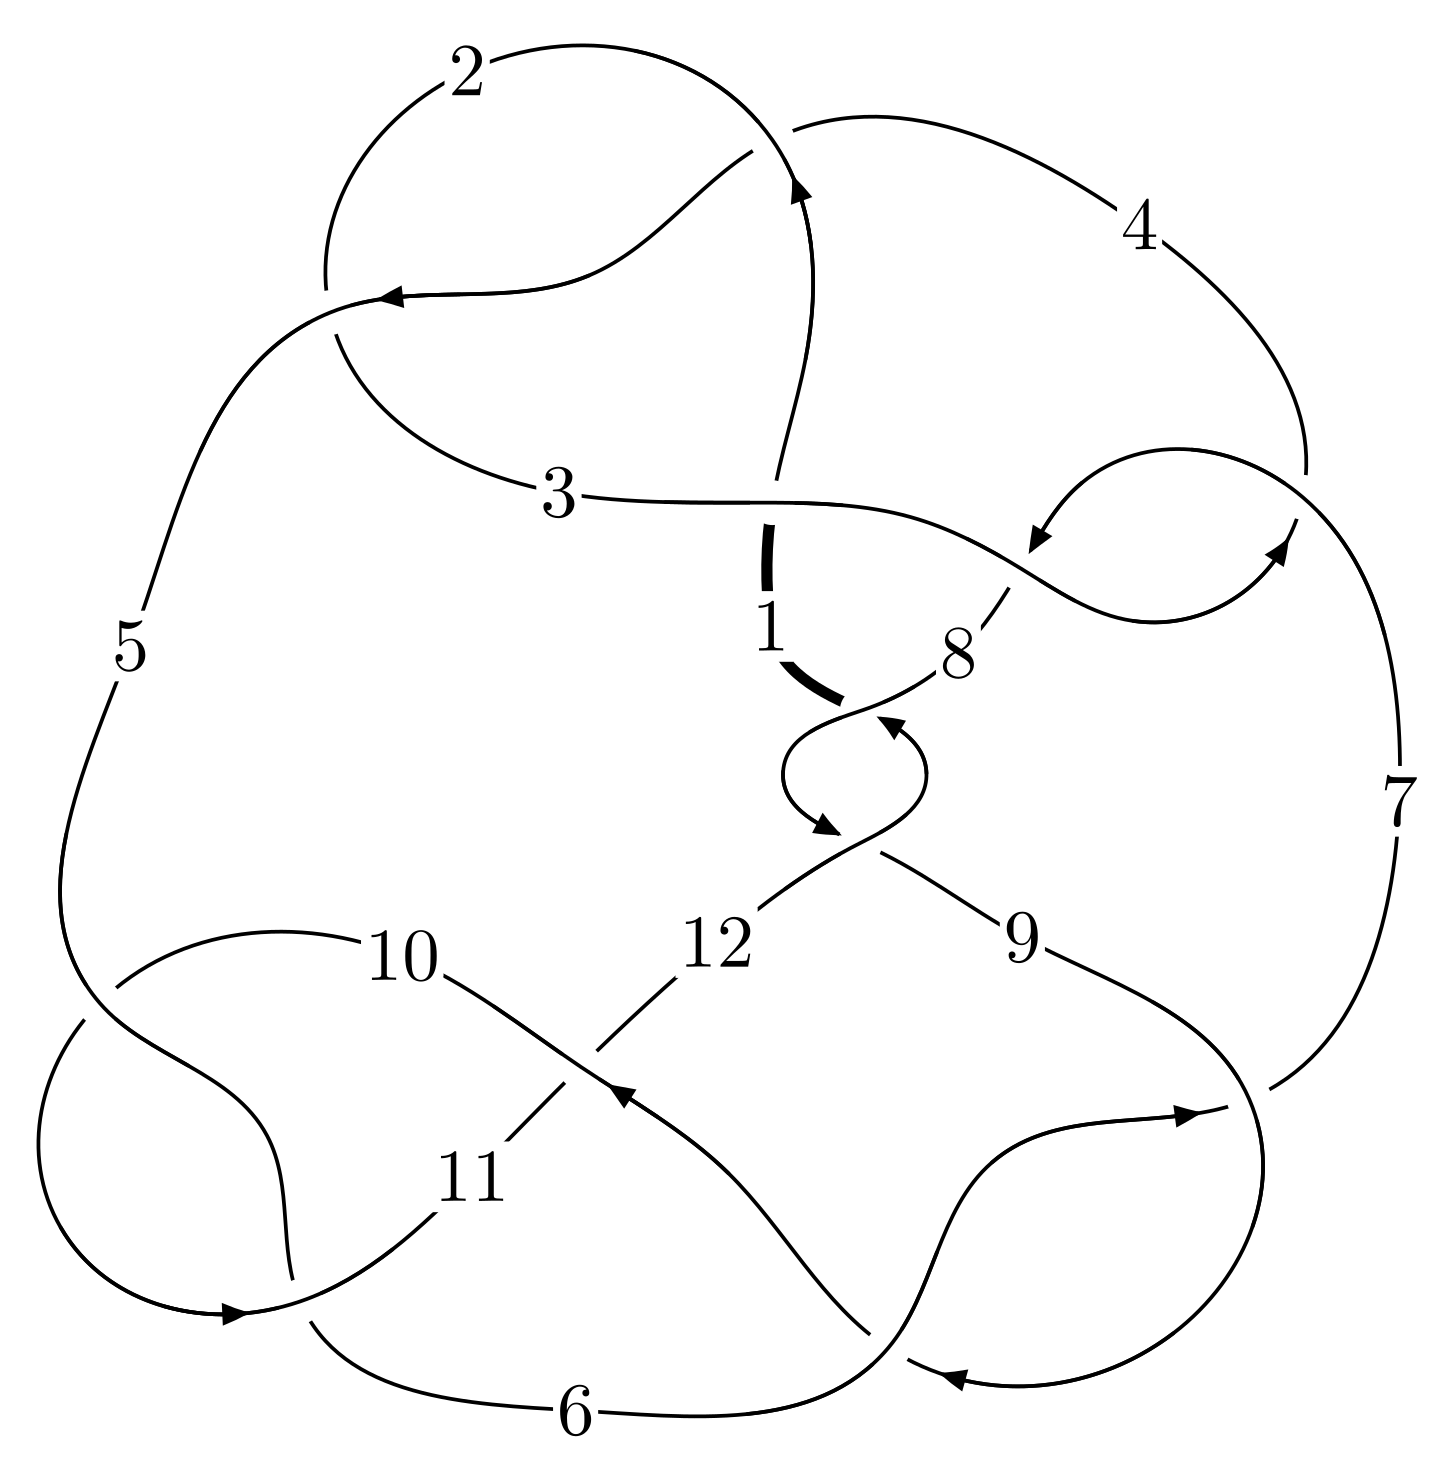
\includegraphics[width=112pt]{../../../GIT/diagram.site/Diagrams/png/2307_12n_0218.png}\\
\ \ \ A knot diagram\footnotemark}&
\allowdisplaybreaks
\textbf{Linearized knot diagam} \\
\cline{2-2}
 &
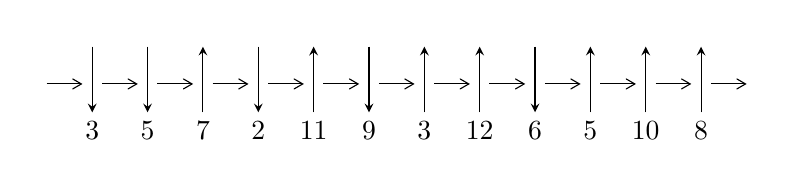
\begin{tikzpicture}[x=20pt, y=17pt]
	% nodes
	\node (C0) at (0, 0) {};
	\node (C1) at (1, 0) {};
	\node (C1U) at (1, +1) {};
	\node (C1D) at (1, -1) {3};

	\node (C2) at (2, 0) {};
	\node (C2U) at (2, +1) {};
	\node (C2D) at (2, -1) {5};

	\node (C3) at (3, 0) {};
	\node (C3U) at (3, +1) {};
	\node (C3D) at (3, -1) {7};

	\node (C4) at (4, 0) {};
	\node (C4U) at (4, +1) {};
	\node (C4D) at (4, -1) {2};

	\node (C5) at (5, 0) {};
	\node (C5U) at (5, +1) {};
	\node (C5D) at (5, -1) {11};

	\node (C6) at (6, 0) {};
	\node (C6U) at (6, +1) {};
	\node (C6D) at (6, -1) {9};

	\node (C7) at (7, 0) {};
	\node (C7U) at (7, +1) {};
	\node (C7D) at (7, -1) {3};

	\node (C8) at (8, 0) {};
	\node (C8U) at (8, +1) {};
	\node (C8D) at (8, -1) {12};

	\node (C9) at (9, 0) {};
	\node (C9U) at (9, +1) {};
	\node (C9D) at (9, -1) {6};

	\node (C10) at (10, 0) {};
	\node (C10U) at (10, +1) {};
	\node (C10D) at (10, -1) {5};

	\node (C11) at (11, 0) {};
	\node (C11U) at (11, +1) {};
	\node (C11D) at (11, -1) {10};

	\node (C12) at (12, 0) {};
	\node (C12U) at (12, +1) {};
	\node (C12D) at (12, -1) {8};
	\node (C13) at (13, 0) {};

	% arrows
	\draw[->,>={angle 60}]
	(C0) edge (C1) (C1) edge (C2) (C2) edge (C3) (C3) edge (C4) (C4) edge (C5) (C5) edge (C6) (C6) edge (C7) (C7) edge (C8) (C8) edge (C9) (C9) edge (C10) (C10) edge (C11) (C11) edge (C12) (C12) edge (C13) ;	\draw[->,>=stealth]
	(C1U) edge (C1D) (C2U) edge (C2D) (C3D) edge (C3U) (C4U) edge (C4D) (C5D) edge (C5U) (C6U) edge (C6D) (C7D) edge (C7U) (C8D) edge (C8U) (C9U) edge (C9D) (C10D) edge (C10U) (C11D) edge (C11U) (C12D) edge (C12U) ;
	\end{tikzpicture} \\
\hhline{~~} \\& 
\textbf{Solving Sequence} \\ \cline{2-2} 
 &
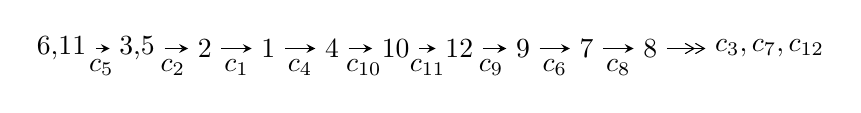
\begin{tikzpicture}[x=23pt, y=7pt]
	% node
	\node (A0) at (-1/8, 0) {6,11};
	\node (A1) at (17/16, 0) {3,5};
	\node (A2) at (17/8, 0) {2};
	\node (A3) at (25/8, 0) {1};
	\node (A4) at (33/8, 0) {4};
	\node (A5) at (41/8, 0) {10};
	\node (A6) at (49/8, 0) {12};
	\node (A7) at (57/8, 0) {9};
	\node (A8) at (65/8, 0) {7};
	\node (A9) at (73/8, 0) {8};
	\node (C1) at (1/2, -1) {$c_{5}$};
	\node (C2) at (13/8, -1) {$c_{2}$};
	\node (C3) at (21/8, -1) {$c_{1}$};
	\node (C4) at (29/8, -1) {$c_{4}$};
	\node (C5) at (37/8, -1) {$c_{10}$};
	\node (C6) at (45/8, -1) {$c_{11}$};
	\node (C7) at (53/8, -1) {$c_{9}$};
	\node (C8) at (61/8, -1) {$c_{6}$};
	\node (C9) at (69/8, -1) {$c_{8}$};
	\node (A10) at (11, 0) {$c_{3},c_{7},c_{12}$};

	% edge
	\draw[->,>=stealth]	
	(A0) edge (A1) (A1) edge (A2) (A2) edge (A3) (A3) edge (A4) (A4) edge (A5) (A5) edge (A6) (A6) edge (A7) (A7) edge (A8) (A8) edge (A9) ;
	\draw[->>,>={angle 60}]	
	(A9) edge (A10);
\end{tikzpicture} \\ 

\end{tabular} \\

\footnotetext{
The image of knot diagram is generated by the software ``\textbf{Draw programme}" developed by Andrew Bartholomew(\url{http://www.layer8.co.uk/maths/draw/index.htm\#Running-draw}), where we modified some parts for our purpose(\url{https://github.com/CATsTAILs/LinksPainter}).
}\phantom \\ \newline 
\centering \textbf{Ideals for irreducible components\footnotemark of $X_{\text{par}}$} 
 
\begin{align*}
I^u_{1}&=\langle 
- u^{22}-2 u^{21}+\cdots+b-1,\;- u^{22}- u^{21}+\cdots+a-1,\;u^{23}+2 u^{22}+\cdots+2 u+1\rangle \\
I^u_{2}&=\langle 
u^8-2 u^6+u^5+2 u^4- u^3+b+u,\;u^7-2 u^5+u^4+2 u^3- u^2+a+u,\\
\phantom{I^u_{2}}&\phantom{= \langle  }u^9- u^8-2 u^7+3 u^6+u^5-3 u^4+2 u^3- u+1\rangle \\
\\
\end{align*}
\raggedright * 2 irreducible components of $\dim_{\mathbb{C}}=0$, with total 32 representations.\\
\footnotetext{All coefficients of polynomials are rational numbers. But the coefficients are sometimes approximated in decimal forms when there is not enough margin.}
\newpage
\renewcommand{\arraystretch}{1}
\centering \section*{I. $I^u_{1}= \langle - u^{22}-2 u^{21}+\cdots+b-1,\;- u^{22}- u^{21}+\cdots+a-1,\;u^{23}+2 u^{22}+\cdots+2 u+1 \rangle$}
\flushleft \textbf{(i) Arc colorings}\\
\begin{tabular}{m{7pt} m{180pt} m{7pt} m{180pt} }
\flushright $a_{6}=$&$\begin{pmatrix}1\\0\end{pmatrix}$ \\
\flushright $a_{11}=$&$\begin{pmatrix}0\\u\end{pmatrix}$ \\
\flushright $a_{3}=$&$\begin{pmatrix}u^{22}+u^{21}+\cdots+2 u+1\\u^{22}+2 u^{21}+\cdots+2 u+1\end{pmatrix}$ \\
\flushright $a_{5}=$&$\begin{pmatrix}1\\u^2\end{pmatrix}$ \\
\flushright $a_{2}=$&$\begin{pmatrix}2 u^{22}+2 u^{21}+\cdots+3 u+1\\2 u^{22}+3 u^{21}+\cdots+3 u+2\end{pmatrix}$ \\
\flushright $a_{1}=$&$\begin{pmatrix}- u^{19}+4 u^{17}-8 u^{15}+8 u^{13}-5 u^{11}+2 u^9-2 u^7- u^3\\- u^{21}+5 u^{19}-13 u^{17}+20 u^{15}-20 u^{13}+11 u^{11}- u^9-4 u^7+u^5+u^3- u\end{pmatrix}$ \\
\flushright $a_{4}=$&$\begin{pmatrix}3 u^{22}+3 u^{21}+\cdots+5 u+2\\3 u^{22}+4 u^{21}+\cdots+5 u+3\end{pmatrix}$ \\
\flushright $a_{10}=$&$\begin{pmatrix}- u\\- u^3+u\end{pmatrix}$ \\
\flushright $a_{12}=$&$\begin{pmatrix}u^3\\u^5- u^3+u\end{pmatrix}$ \\
\flushright $a_{9}=$&$\begin{pmatrix}- u^3\\- u^3+u\end{pmatrix}$ \\
\flushright $a_{7}=$&$\begin{pmatrix}u^6- u^4+1\\u^6-2 u^4+u^2\end{pmatrix}$ \\
\flushright $a_{8}=$&$\begin{pmatrix}- u^{11}+2 u^9-2 u^7- u^3\\- u^{13}+3 u^{11}-5 u^9+4 u^7-2 u^5- u^3+u\end{pmatrix}$\\&\end{tabular}
\flushleft \textbf{(ii) Obstruction class $= -1$}\\~\\
\flushleft \textbf{(iii) Cusp Shapes $= 10 u^{22}+11 u^{21}-52 u^{20}-76 u^{19}+117 u^{18}+231 u^{17}-102 u^{16}-390 u^{15}-69 u^{14}+358 u^{13}+268 u^{12}-113 u^{11}-261 u^{10}-92 u^9+98 u^8+84 u^7+19 u^6+10 u^5-11 u^4-33 u^3- u^2+12 u+11$}\\~\\
\newpage\renewcommand{\arraystretch}{1}
\flushleft \textbf{(iv) u-Polynomials at the component}\newline \\
\begin{tabular}{m{50pt}|m{274pt}}
Crossings & \hspace{64pt}u-Polynomials at each crossing \\
\hline $$\begin{aligned}c_{1}\end{aligned}$$&$\begin{aligned}
&u^{23}+44 u^{22}+\cdots+46 u+1
\end{aligned}$\\
\hline $$\begin{aligned}c_{2},c_{4}\end{aligned}$$&$\begin{aligned}
&u^{23}-10 u^{22}+\cdots+10 u-1
\end{aligned}$\\
\hline $$\begin{aligned}c_{3},c_{7}\end{aligned}$$&$\begin{aligned}
&u^{23}- u^{22}+\cdots+512 u-512
\end{aligned}$\\
\hline $$\begin{aligned}c_{5},c_{10}\end{aligned}$$&$\begin{aligned}
&u^{23}-2 u^{22}+\cdots+2 u-1
\end{aligned}$\\
\hline $$\begin{aligned}c_{6},c_{9}\end{aligned}$$&$\begin{aligned}
&u^{23}-6 u^{22}+\cdots+30 u-7
\end{aligned}$\\
\hline $$\begin{aligned}c_{8},c_{12}\end{aligned}$$&$\begin{aligned}
&u^{23}+24 u^{21}+\cdots+2 u-1
\end{aligned}$\\
\hline $$\begin{aligned}c_{11}\end{aligned}$$&$\begin{aligned}
&u^{23}-12 u^{22}+\cdots+2 u-1
\end{aligned}$\\
\hline
\end{tabular}\\~\\
\newpage\renewcommand{\arraystretch}{1}
\flushleft \textbf{(v) Riley Polynomials at the component}\newline \\
\begin{tabular}{m{50pt}|m{274pt}}
Crossings & \hspace{64pt}Riley Polynomials at each crossing \\
\hline $$\begin{aligned}c_{1}\end{aligned}$$&$\begin{aligned}
&y^{23}-168 y^{22}+\cdots+3538 y-1
\end{aligned}$\\
\hline $$\begin{aligned}c_{2},c_{4}\end{aligned}$$&$\begin{aligned}
&y^{23}-44 y^{22}+\cdots+46 y-1
\end{aligned}$\\
\hline $$\begin{aligned}c_{3},c_{7}\end{aligned}$$&$\begin{aligned}
&y^{23}+57 y^{22}+\cdots+2621440 y-262144
\end{aligned}$\\
\hline $$\begin{aligned}c_{5},c_{10}\end{aligned}$$&$\begin{aligned}
&y^{23}-12 y^{22}+\cdots+2 y-1
\end{aligned}$\\
\hline $$\begin{aligned}c_{6},c_{9}\end{aligned}$$&$\begin{aligned}
&y^{23}+12 y^{22}+\cdots+410 y-49
\end{aligned}$\\
\hline $$\begin{aligned}c_{8},c_{12}\end{aligned}$$&$\begin{aligned}
&y^{23}+48 y^{22}+\cdots+2 y-1
\end{aligned}$\\
\hline $$\begin{aligned}c_{11}\end{aligned}$$&$\begin{aligned}
&y^{23}+24 y^{21}+\cdots-2 y-1
\end{aligned}$\\
\hline
\end{tabular}\\~\\
\newpage\flushleft \textbf{(vi) Complex Volumes and Cusp Shapes}
$$\begin{array}{c|c|c}  
\text{Solutions to }I^u_{1}& \I (\text{vol} + \sqrt{-1}CS) & \text{Cusp shape}\\
 \hline 
\begin{aligned}
u &= -0.793555 + 0.695238 I \\
a &= \phantom{-}0.27094 - 1.56138 I \\
b &= \phantom{-}0.563681 - 0.478675 I\end{aligned}
 & \phantom{-}19.5669 - 2.6314 I & -2.85971 + 2.82212 I \\ \hline\begin{aligned}
u &= -0.793555 - 0.695238 I \\
a &= \phantom{-}0.27094 + 1.56138 I \\
b &= \phantom{-}0.563681 + 0.478675 I\end{aligned}
 & \phantom{-}19.5669 + 2.6314 I & -2.85971 - 2.82212 I \\ \hline\begin{aligned}
u &= \phantom{-}1.022100 + 0.407841 I \\
a &= \phantom{-}1.44074 + 0.54244 I \\
b &= -0.140040 + 1.113520 I\end{aligned}
 & \phantom{-}0.05293 + 1.76634 I & \phantom{-}1.02070 - 2.91905 I \\ \hline\begin{aligned}
u &= \phantom{-}1.022100 - 0.407841 I \\
a &= \phantom{-}1.44074 - 0.54244 I \\
b &= -0.140040 - 1.113520 I\end{aligned}
 & \phantom{-}0.05293 - 1.76634 I & \phantom{-}1.02070 + 2.91905 I \\ \hline\begin{aligned}
u &= -0.260502 + 0.851460 I \\
a &= -0.101202 + 0.883554 I \\
b &= \phantom{-}2.59298 - 0.76044 I\end{aligned}
 & -16.8734 + 5.0391 I & -2.11769 - 1.80422 I \\ \hline\begin{aligned}
u &= -0.260502 - 0.851460 I \\
a &= -0.101202 - 0.883554 I \\
b &= \phantom{-}2.59298 + 0.76044 I\end{aligned}
 & -16.8734 - 5.0391 I & -2.11769 + 1.80422 I \\ \hline\begin{aligned}
u &= -1.072240 + 0.511021 I \\
a &= \phantom{-}0.05623 + 2.46640 I \\
b &= \phantom{-}1.31169 + 1.69266 I\end{aligned}
 & -0.80606 - 4.86361 I & \phantom{-}0.58399 + 4.58744 I \\ \hline\begin{aligned}
u &= -1.072240 - 0.511021 I \\
a &= \phantom{-}0.05623 - 2.46640 I \\
b &= \phantom{-}1.31169 - 1.69266 I\end{aligned}
 & -0.80606 + 4.86361 I & \phantom{-}0.58399 - 4.58744 I \\ \hline\begin{aligned}
u &= -1.151200 + 0.397103 I \\
a &= \phantom{-}0.378436 - 0.814303 I \\
b &= -0.061499 - 0.968355 I\end{aligned}
 & \phantom{-}4.03412 - 1.87941 I & \phantom{-}8.76933 + 1.17253 I \\ \hline\begin{aligned}
u &= -1.151200 - 0.397103 I \\
a &= \phantom{-}0.378436 + 0.814303 I \\
b &= -0.061499 + 0.968355 I\end{aligned}
 & \phantom{-}4.03412 + 1.87941 I & \phantom{-}8.76933 - 1.17253 I\\
 \hline 
 \end{array}$$\newpage$$\begin{array}{c|c|c}  
\text{Solutions to }I^u_{1}& \I (\text{vol} + \sqrt{-1}CS) & \text{Cusp shape}\\
 \hline 
\begin{aligned}
u &= \phantom{-}0.669270 + 0.402839 I \\
a &= \phantom{-}0.378364 - 0.834298 I \\
b &= \phantom{-}0.169751 + 0.377973 I\end{aligned}
 & -1.04289 + 1.55239 I & -1.64388 - 5.32889 I \\ \hline\begin{aligned}
u &= \phantom{-}0.669270 - 0.402839 I \\
a &= \phantom{-}0.378364 + 0.834298 I \\
b &= \phantom{-}0.169751 - 0.377973 I\end{aligned}
 & -1.04289 - 1.55239 I & -1.64388 + 5.32889 I \\ \hline\begin{aligned}
u &= -0.769798\phantom{ +0.000000I} \\
a &= \phantom{-}0.600191\phantom{ +0.000000I} \\
b &= \phantom{-}0.484933\phantom{ +0.000000I}\end{aligned}
 & \phantom{-}1.02417\phantom{ +0.000000I} & \phantom{-}10.8970\phantom{ +0.000000I} \\ \hline\begin{aligned}
u &= \phantom{-}1.151500 + 0.497191 I \\
a &= -0.371757 - 0.631221 I \\
b &= \phantom{-}0.523099 - 0.584172 I\end{aligned}
 & \phantom{-}3.31594 + 6.22870 I & \phantom{-}6.08610 - 5.76635 I \\ \hline\begin{aligned}
u &= \phantom{-}1.151500 - 0.497191 I \\
a &= -0.371757 + 0.631221 I \\
b &= \phantom{-}0.523099 + 0.584172 I\end{aligned}
 & \phantom{-}3.31594 - 6.22870 I & \phantom{-}6.08610 + 5.76635 I \\ \hline\begin{aligned}
u &= \phantom{-}1.233100 + 0.274609 I \\
a &= -2.75962 + 0.02500 I \\
b &= -1.94681 - 1.66946 I\end{aligned}
 & -12.07890 - 1.46711 I & \phantom{-}2.75909 - 0.30473 I \\ \hline\begin{aligned}
u &= \phantom{-}1.233100 - 0.274609 I \\
a &= -2.75962 - 0.02500 I \\
b &= -1.94681 + 1.66946 I\end{aligned}
 & -12.07890 + 1.46711 I & \phantom{-}2.75909 + 0.30473 I \\ \hline\begin{aligned}
u &= \phantom{-}0.152344 + 0.678389 I \\
a &= \phantom{-}0.370495 + 0.387642 I \\
b &= -0.142963 - 0.519552 I\end{aligned}
 & \phantom{-}0.49322 - 1.74871 I & \phantom{-}2.97942 + 3.32574 I \\ \hline\begin{aligned}
u &= \phantom{-}0.152344 - 0.678389 I \\
a &= \phantom{-}0.370495 - 0.387642 I \\
b &= -0.142963 + 0.519552 I\end{aligned}
 & \phantom{-}0.49322 + 1.74871 I & \phantom{-}2.97942 - 3.32574 I \\ \hline\begin{aligned}
u &= -1.179040 + 0.569666 I \\
a &= -1.36258 - 2.90160 I \\
b &= -3.23838 - 0.97939 I\end{aligned}
 & -14.1285 - 10.2729 I & \phantom{-}0.79116 + 5.29982 I\\
 \hline 
 \end{array}$$\newpage$$\begin{array}{c|c|c}  
\text{Solutions to }I^u_{1}& \I (\text{vol} + \sqrt{-1}CS) & \text{Cusp shape}\\
 \hline 
\begin{aligned}
u &= -1.179040 - 0.569666 I \\
a &= -1.36258 + 2.90160 I \\
b &= -3.23838 + 0.97939 I\end{aligned}
 & -14.1285 + 10.2729 I & \phantom{-}0.79116 - 5.29982 I \\ \hline\begin{aligned}
u &= -0.386868 + 0.554823 I \\
a &= -1.100140 - 0.404039 I \\
b &= -1.37398 + 0.73498 I\end{aligned}
 & -2.78460 + 0.52794 I & -2.81721 + 0.26390 I \\ \hline\begin{aligned}
u &= -0.386868 - 0.554823 I \\
a &= -1.100140 + 0.404039 I \\
b &= -1.37398 - 0.73498 I\end{aligned}
 & -2.78460 - 0.52794 I & -2.81721 - 0.26390 I\\
 \hline 
 \end{array}$$\newpage\newpage\renewcommand{\arraystretch}{1}
\centering \section*{II. $I^u_{2}= \langle u^8-2 u^6+u^5+2 u^4- u^3+b+u,\;u^7-2 u^5+u^4+2 u^3- u^2+a+u,\;u^9- u^8-2 u^7+3 u^6+u^5-3 u^4+2 u^3- u+1 \rangle$}
\flushleft \textbf{(i) Arc colorings}\\
\begin{tabular}{m{7pt} m{180pt} m{7pt} m{180pt} }
\flushright $a_{6}=$&$\begin{pmatrix}1\\0\end{pmatrix}$ \\
\flushright $a_{11}=$&$\begin{pmatrix}0\\u\end{pmatrix}$ \\
\flushright $a_{3}=$&$\begin{pmatrix}- u^7+2 u^5- u^4-2 u^3+u^2- u\\- u^8+2 u^6- u^5-2 u^4+u^3- u\end{pmatrix}$ \\
\flushright $a_{5}=$&$\begin{pmatrix}1\\u^2\end{pmatrix}$ \\
\flushright $a_{2}=$&$\begin{pmatrix}- u^7+2 u^5- u^4-2 u^3+u^2- u-1\\- u^8+2 u^6- u^5-2 u^4+u^3- u^2- u\end{pmatrix}$ \\
\flushright $a_{1}=$&$\begin{pmatrix}-1\\- u^2\end{pmatrix}$ \\
\flushright $a_{4}=$&$\begin{pmatrix}- u^7+2 u^5- u^4-2 u^3+u^2- u\\- u^8+2 u^6- u^5-2 u^4+u^3- u\end{pmatrix}$ \\
\flushright $a_{10}=$&$\begin{pmatrix}- u\\- u^3+u\end{pmatrix}$ \\
\flushright $a_{12}=$&$\begin{pmatrix}u^3\\u^5- u^3+u\end{pmatrix}$ \\
\flushright $a_{9}=$&$\begin{pmatrix}- u^3\\- u^3+u\end{pmatrix}$ \\
\flushright $a_{7}=$&$\begin{pmatrix}u^6- u^4+1\\u^6-2 u^4+u^2\end{pmatrix}$ \\
\flushright $a_{8}=$&$\begin{pmatrix}u^6- u^4+1\\u^6-2 u^4+u^2\end{pmatrix}$\\&\end{tabular}
\flushleft \textbf{(ii) Obstruction class $= 1$}\\~\\
\flushleft \textbf{(iii) Cusp Shapes $= - u^8-2 u^7+u^6+4 u^5-3 u^4-6 u^3+u^2- u-2$}\\~\\
\newpage\renewcommand{\arraystretch}{1}
\flushleft \textbf{(iv) u-Polynomials at the component}\newline \\
\begin{tabular}{m{50pt}|m{274pt}}
Crossings & \hspace{64pt}u-Polynomials at each crossing \\
\hline $$\begin{aligned}c_{1},c_{2}\end{aligned}$$&$\begin{aligned}
&(u-1)^9
\end{aligned}$\\
\hline $$\begin{aligned}c_{3},c_{7}\end{aligned}$$&$\begin{aligned}
&u^9
\end{aligned}$\\
\hline $$\begin{aligned}c_{4}\end{aligned}$$&$\begin{aligned}
&(u+1)^9
\end{aligned}$\\
\hline $$\begin{aligned}c_{5}\end{aligned}$$&$\begin{aligned}
&u^9- u^8-2 u^7+3 u^6+u^5-3 u^4+2 u^3- u+1
\end{aligned}$\\
\hline $$\begin{aligned}c_{6}\end{aligned}$$&$\begin{aligned}
&u^9-3 u^8+8 u^7-13 u^6+17 u^5-17 u^4+12 u^3-6 u^2+u+1
\end{aligned}$\\
\hline $$\begin{aligned}c_{8}\end{aligned}$$&$\begin{aligned}
&u^9- u^8+2 u^7- u^6+3 u^5- u^4+2 u^3+u+1
\end{aligned}$\\
\hline $$\begin{aligned}c_{9}\end{aligned}$$&$\begin{aligned}
&u^9+3 u^8+8 u^7+13 u^6+17 u^5+17 u^4+12 u^3+6 u^2+u-1
\end{aligned}$\\
\hline $$\begin{aligned}c_{10}\end{aligned}$$&$\begin{aligned}
&u^9+u^8-2 u^7-3 u^6+u^5+3 u^4+2 u^3- u-1
\end{aligned}$\\
\hline $$\begin{aligned}c_{11}\end{aligned}$$&$\begin{aligned}
&u^9-5 u^8+12 u^7-15 u^6+9 u^5+u^4-4 u^3+2 u^2+u-1
\end{aligned}$\\
\hline $$\begin{aligned}c_{12}\end{aligned}$$&$\begin{aligned}
&u^9+u^8+2 u^7+u^6+3 u^5+u^4+2 u^3+u-1
\end{aligned}$\\
\hline
\end{tabular}\\~\\
\newpage\renewcommand{\arraystretch}{1}
\flushleft \textbf{(v) Riley Polynomials at the component}\newline \\
\begin{tabular}{m{50pt}|m{274pt}}
Crossings & \hspace{64pt}Riley Polynomials at each crossing \\
\hline $$\begin{aligned}c_{1},c_{2},c_{4}\end{aligned}$$&$\begin{aligned}
&(y-1)^9
\end{aligned}$\\
\hline $$\begin{aligned}c_{3},c_{7}\end{aligned}$$&$\begin{aligned}
&y^9
\end{aligned}$\\
\hline $$\begin{aligned}c_{5},c_{10}\end{aligned}$$&$\begin{aligned}
&y^9-5 y^8+12 y^7-15 y^6+9 y^5+y^4-4 y^3+2 y^2+y-1
\end{aligned}$\\
\hline $$\begin{aligned}c_{6},c_{9}\end{aligned}$$&$\begin{aligned}
&y^9+7 y^8+20 y^7+25 y^6+5 y^5-15 y^4+22 y^2+13 y-1
\end{aligned}$\\
\hline $$\begin{aligned}c_{8},c_{12}\end{aligned}$$&$\begin{aligned}
&y^9+3 y^8+8 y^7+13 y^6+17 y^5+17 y^4+12 y^3+6 y^2+y-1
\end{aligned}$\\
\hline $$\begin{aligned}c_{11}\end{aligned}$$&$\begin{aligned}
&y^9- y^8+12 y^7-7 y^6+37 y^5+y^4-10 y^2+5 y-1
\end{aligned}$\\
\hline
\end{tabular}\\~\\
\newpage\flushleft \textbf{(vi) Complex Volumes and Cusp Shapes}
$$\begin{array}{c|c|c}  
\text{Solutions to }I^u_{2}& \I (\text{vol} + \sqrt{-1}CS) & \text{Cusp shape}\\
 \hline 
\begin{aligned}
u &= \phantom{-}0.772920 + 0.510351 I \\
a &= -0.628748 - 1.040710 I \\
b &= -0.390818 - 0.846696 I\end{aligned}
 & -3.42837 + 2.09337 I & -2.59545 - 4.13635 I \\ \hline\begin{aligned}
u &= \phantom{-}0.772920 - 0.510351 I \\
a &= -0.628748 + 1.040710 I \\
b &= -0.390818 + 0.846696 I\end{aligned}
 & -3.42837 - 2.09337 I & -2.59545 + 4.13635 I \\ \hline\begin{aligned}
u &= -0.825933\phantom{ +0.000000I} \\
a &= \phantom{-}1.66309\phantom{ +0.000000I} \\
b &= \phantom{-}0.134499\phantom{ +0.000000I}\end{aligned}
 & -0.446489\phantom{ +0.000000I} & \phantom{-}0.580470\phantom{ +0.000000I} \\ \hline\begin{aligned}
u &= -1.173910 + 0.391555 I \\
a &= \phantom{-}1.321020 + 0.175437 I \\
b &= \phantom{-}0.779205 - 0.999551 I\end{aligned}
 & \phantom{-}2.72642 - 1.33617 I & \phantom{-}3.11790 + 0.38556 I \\ \hline\begin{aligned}
u &= -1.173910 - 0.391555 I \\
a &= \phantom{-}1.321020 - 0.175437 I \\
b &= \phantom{-}0.779205 + 0.999551 I\end{aligned}
 & \phantom{-}2.72642 + 1.33617 I & \phantom{-}3.11790 - 0.38556 I \\ \hline\begin{aligned}
u &= \phantom{-}0.141484 + 0.739668 I \\
a &= \phantom{-}0.081981 + 0.728244 I \\
b &= -1.195640 - 0.366692 I\end{aligned}
 & -1.02799 - 2.45442 I & -1.02595 + 3.19656 I \\ \hline\begin{aligned}
u &= \phantom{-}0.141484 - 0.739668 I \\
a &= \phantom{-}0.081981 - 0.728244 I \\
b &= -1.195640 + 0.366692 I\end{aligned}
 & -1.02799 + 2.45442 I & -1.02595 - 3.19656 I \\ \hline\begin{aligned}
u &= \phantom{-}1.172470 + 0.500383 I \\
a &= \phantom{-}0.89420 - 1.47834 I \\
b &= \phantom{-}1.74000 - 0.61288 I\end{aligned}
 & \phantom{-}1.95319 + 7.08493 I & \phantom{-}2.21327 - 6.71575 I \\ \hline\begin{aligned}
u &= \phantom{-}1.172470 - 0.500383 I \\
a &= \phantom{-}0.89420 + 1.47834 I \\
b &= \phantom{-}1.74000 + 0.61288 I\end{aligned}
 & \phantom{-}1.95319 - 7.08493 I & \phantom{-}2.21327 + 6.71575 I\\
 \hline 
 \end{array}$$\newpage
\newpage\renewcommand{\arraystretch}{1}
\centering \section*{ III. u-Polynomials}
\begin{tabular}{m{50pt}|m{274pt}}
Crossings & \hspace{64pt}u-Polynomials at each crossing \\
\hline $$\begin{aligned}c_{1}\end{aligned}$$&$\begin{aligned}
&((u-1)^9)(u^{23}+44 u^{22}+\cdots+46 u+1)
\end{aligned}$\\
\hline $$\begin{aligned}c_{2}\end{aligned}$$&$\begin{aligned}
&((u-1)^9)(u^{23}-10 u^{22}+\cdots+10 u-1)
\end{aligned}$\\
\hline $$\begin{aligned}c_{3},c_{7}\end{aligned}$$&$\begin{aligned}
&u^9(u^{23}- u^{22}+\cdots+512 u-512)
\end{aligned}$\\
\hline $$\begin{aligned}c_{4}\end{aligned}$$&$\begin{aligned}
&((u+1)^9)(u^{23}-10 u^{22}+\cdots+10 u-1)
\end{aligned}$\\
\hline $$\begin{aligned}c_{5}\end{aligned}$$&$\begin{aligned}
&(u^9- u^8+\cdots- u+1)(u^{23}-2 u^{22}+\cdots+2 u-1)
\end{aligned}$\\
\hline $$\begin{aligned}c_{6}\end{aligned}$$&$\begin{aligned}
&(u^9-3 u^8+8 u^7-13 u^6+17 u^5-17 u^4+12 u^3-6 u^2+u+1)\\
&\cdot(u^{23}-6 u^{22}+\cdots+30 u-7)
\end{aligned}$\\
\hline $$\begin{aligned}c_{8}\end{aligned}$$&$\begin{aligned}
&(u^9- u^8+\cdots+u+1)(u^{23}+24 u^{21}+\cdots+2 u-1)
\end{aligned}$\\
\hline $$\begin{aligned}c_{9}\end{aligned}$$&$\begin{aligned}
&(u^9+3 u^8+8 u^7+13 u^6+17 u^5+17 u^4+12 u^3+6 u^2+u-1)\\
&\cdot(u^{23}-6 u^{22}+\cdots+30 u-7)
\end{aligned}$\\
\hline $$\begin{aligned}c_{10}\end{aligned}$$&$\begin{aligned}
&(u^9+u^8+\cdots- u-1)(u^{23}-2 u^{22}+\cdots+2 u-1)
\end{aligned}$\\
\hline $$\begin{aligned}c_{11}\end{aligned}$$&$\begin{aligned}
&(u^9-5 u^8+12 u^7-15 u^6+9 u^5+u^4-4 u^3+2 u^2+u-1)\\
&\cdot(u^{23}-12 u^{22}+\cdots+2 u-1)
\end{aligned}$\\
\hline $$\begin{aligned}c_{12}\end{aligned}$$&$\begin{aligned}
&(u^9+u^8+\cdots+u-1)(u^{23}+24 u^{21}+\cdots+2 u-1)
\end{aligned}$\\
\hline
\end{tabular}\newpage\renewcommand{\arraystretch}{1}
\centering \section*{ IV. Riley Polynomials}
\begin{tabular}{m{50pt}|m{274pt}}
Crossings & \hspace{64pt}Riley Polynomials at each crossing \\
\hline $$\begin{aligned}c_{1}\end{aligned}$$&$\begin{aligned}
&((y-1)^9)(y^{23}-168 y^{22}+\cdots+3538 y-1)
\end{aligned}$\\
\hline $$\begin{aligned}c_{2},c_{4}\end{aligned}$$&$\begin{aligned}
&((y-1)^9)(y^{23}-44 y^{22}+\cdots+46 y-1)
\end{aligned}$\\
\hline $$\begin{aligned}c_{3},c_{7}\end{aligned}$$&$\begin{aligned}
&y^9(y^{23}+57 y^{22}+\cdots+2621440 y-262144)
\end{aligned}$\\
\hline $$\begin{aligned}c_{5},c_{10}\end{aligned}$$&$\begin{aligned}
&(y^9-5 y^8+12 y^7-15 y^6+9 y^5+y^4-4 y^3+2 y^2+y-1)\\
&\cdot(y^{23}-12 y^{22}+\cdots+2 y-1)
\end{aligned}$\\
\hline $$\begin{aligned}c_{6},c_{9}\end{aligned}$$&$\begin{aligned}
&(y^9+7 y^8+20 y^7+25 y^6+5 y^5-15 y^4+22 y^2+13 y-1)\\
&\cdot(y^{23}+12 y^{22}+\cdots+410 y-49)
\end{aligned}$\\
\hline $$\begin{aligned}c_{8},c_{12}\end{aligned}$$&$\begin{aligned}
&(y^9+3 y^8+8 y^7+13 y^6+17 y^5+17 y^4+12 y^3+6 y^2+y-1)\\
&\cdot(y^{23}+48 y^{22}+\cdots+2 y-1)
\end{aligned}$\\
\hline $$\begin{aligned}c_{11}\end{aligned}$$&$\begin{aligned}
&(y^9- y^8+12 y^7-7 y^6+37 y^5+y^4-10 y^2+5 y-1)\\
&\cdot(y^{23}+24 y^{21}+\cdots-2 y-1)
\end{aligned}$\\
\hline
\end{tabular}
\vskip 2pc
\end{document}